\documentclass[11pt,a4paper]{article}
\setlength{\headheight}{34pt}
\usepackage[margin=1.2in]{geometry}
\usepackage[T1]{fontenc}
\usepackage[utf8]{inputenc}
\usepackage[german]{babel}
\usepackage[printonlyused]{acronym}
\usepackage[
	colorlinks=false,
	urlcolor=blue,
	linkcolor= gray
]{hyperref}
\usepackage{lmodern,textcomp}
\usepackage{graphicx}
\usepackage{pdfpages}
\graphicspath{ {images/} }
\usepackage{amsmath}
\usepackage{svg}
\usepackage{amsfonts}
\usepackage{amssymb}
\usepackage{fancyhdr}
\pagestyle{fancy}
\fancyhf{}
\rhead{
\includegraphics[scale=0.05]{logo_zmb}}
\lhead{\textbf{Agentur Website}\\Ein Full Stack Webdevelopement Projekt}
\rfoot{Seite \thepage}
\author{Jeremy Seipelt}
\title{IHK Abschluss-Projekt 2017}
\begin{document}
\clearpage\maketitle
\thispagestyle{empty}
	\begin{center}
		\begin{Large}
		
			
			Für den Beruf des Fachinformatiker der Anwendungsentwicklung\\
			
		\end{Large}
	\end{center}
 
 	\begin{center}
		\begin{LARGE}
			 \textbf{Agentur Website}\\			 
		 Ein Full-Stack Web-Developer Projekt
		\end{LARGE}
	\end{center}
	
	\begin{center}
	Auszubbildner: \\ 
 	Jeremy Seipelt\\
 	Pichelsdorferstr. 72\\
	 13595 Berlin\\
	\end{center}	
	
	\begin{center}
		
\includegraphics[scale=0.05]{logo_zmb}\\
 		Ausbildungsbetrieb:\\
 		zmb GmbH\\
 		Scharnhorstr. 112\\
 		11234 Berlin \\
 	\end{center}
\newpage
\tableofcontents
\newpage
\begin{acronym}[Full Stack]
 \acro{SSR}{Server Sided Rendering}
 \acro{SSA}{Single Site Application}
 \acro{DOM}{Document Object Model}
\end{acronym}
\begin{acronym}[Allgemein]
 \acro{B2B}{Business to Business}
 \acro{KMU}{Kleines Mittelständisches Unternehmen}
\end{acronym}
\newpage
\setcounter{page}{1}
\section{Vorwort}
Diese Projektdokumentation ist für die Abschlussprüfung der IHK für den Beruf des Fachinformatikers der Anwendungsentwicklung entstanden und beschreibt Vorgehensweisen des Verfassers.\\
Ausbildungsbetrieb ist die zmb GmbH, ein KMU mit Standort in Berlin Mitte.
Die zmb vertreibt ihre eigen E-Commerce Plattform, genannt CORE, und geht Projektarbeiten im \acs{B2B} Bereich für alle gängigen Shopsysteme nach.  
Dabei legt die zmb Wert darauf alle Wünsche des Kunden, von der Bereitstellung eigener API über Onboarding bis hin zu Zahlungsweisen, zu erfüllen. 
\subsection{Beschreibung des Projektes}
Für die neu geplanten Agenturarbeiten der zmb, soll eine neue Internet-Präsenz aufgebaut werden.\\\\
Die zmb wird zurzeit nur durch eine Website aus statischen Seiten, die durch das interne CMS System gepflegt werden, präsentiert, sowie auf Partnerseiten.\\\\
Die neue Seite wird eine \acs{SSA} um die Seite für den Kunden modern und schnell zu machen.  
Der Server muss dafür die \acs{SSA} bereits kompiliert versenden, da Suchmaschinen sich nur die gesendete HTML Datei ansehen, dafür benötigen wird ein \acs{SSR}-Setup auf dem Server.
Dafür wird im Verlauf des Projekts ein Server gemietet sowie aufgesetzt. Und eine Website erstellt auf der potentielle Kunden mit der zmb in Kontakt treten können.  
\subsection{Ziel des Projektes}
Am Ende des Projekts soll eine \acs{SSA} entstehen die mithilfe von \acs{SSR} auch ein Vernünftiges SEO Ranking hinbekommt. Dabei sollen namenhafte Geschwindigkeitsindexe die Seite mit maximalen Punkten bewerten.
Die Inhalte der \acs{SSA} werden über ein selbst auf dem Server installiertes CMS-System eingetragen.
Am Ende entsteht somit eine Website die auch ohne Hilfe von HTML sowie JS und CSS gepflegt werden kann.
\subsection{Umfeld des Projektes}
Das Projekt wurde vom COO Simeon Gerodetti beantragt.\\
Herr Gerodetti ist in der zmb für das operative Geschäft sowie für das Marketing, den Online-Auftritt der zmb zuständig.
Des weiteren kümmert er sich um die Partner im \acs{B2B} Bereich und sorgt für Kundenaufträge und das Rechnungswesen des Unternehmens.\\\\
Jovan Gerodetti ist der Softwareentwickler für Frontend sowie der Spezialist in Angular. Er baut neue UIs sowie Schnittstellen für CORE und stellt eine Beratende Funktion für das Projekt dar.\\\\
Für das Projekt ist S. Gerodetti für Entscheidungen im Design und J. Gerodetti bei Fragen zur Implementierung zuständig.\\
Die Abnahme des Projektes wird von S. Gerodetti vollzogen.
\subsection{Projektentscheidung}
Das Hauptgeschäft besteht aus dem Verkauf und der Entwicklung der Inhouse E-Commerce Lösung 'CORE', welche von 3 Personen gewartet wird. 'Core' wird bisher nur als SaaS Lösung eingesetzt und deshalb liegt der administrative Aufwand bei der zmb. Deswegen wird geplant von der eigenen Lösung wegzugehen und den Kunden, für bereits vorhandene Shopsysteme, Lösungen anzubieten.\\\\
Den ersten Schritt in die Richtung der Agenturarbeit geht die zmb mit der zmb.agency Website, dessen Unterbau durch dieses Projekt entsteht.
\subsection{Beschränkungen des Projektes}
Das Projekt beschränkt sich auf das Aufsetzen sowie implementieren einer kleineren Version der Agentur Website die schon alle technischen Voraussetzungen und ein Bruchteil des Inhaltes enthält. Deswegen wird der Großteil der Layout und CSS Arbeiten die im größeren Umfang ein Teil sind, sowie das Anlegen von Inhalten für die Seite, nicht in die Projektzeit eingerechnet.\\
Probleme die zur Verzögerung des ganzen Projekts geführt hätten wurden aus der Projektplanung ausgenommen. (Ausführen)
\section{Projekt-Planung}
Das Projekt wurde auf 70h für die Anforderungen der IHK angesetzt. 
\subsection{Projektverlauf}
Ein Übersicht der Hauptphasen sind der Tabelle 1 zu entnehmen. Eine detaillierte Ansicht der Zeitplanung ist in der \ref{sec:teilaufg} auf Seite \pageref{sec:teilaufg} hinterlegt.\\
\begin{table}[!ht]
  \centering
     \begin{tabular}{l|r}
       \textbf{Phase}  & \textbf{Dauer in Stunden} \\
       \hline
      Analyse       & 8                     \\
      Entwurf       & 7             	    \\
      Implementierung       & 23	\\
      Testen       & 13			         \\
       Dokumentation      &  8        \\
       \hline
       \hline
       Gesammt        & 64               \\
     \end{tabular}
     \caption{Übersicht der Zeitplanung}
\label{tbl:Übersicht der Zeitplanung}
\end{table} 
\subsection{Ressourcenplanung}
Bei der Auswahl der Ressourcen wurde Wert auf Open Source Lösungen wert gelegt, um Projektkosten möglichst gering zu halten. Die Liste aller Benutzter Software ist unter %Todo
zu finden.
\subsection{Entwicklungsprozess}
Die Entwicklung der Website wird per Wasserfall-Modell abgewickelt. Dabei werden die einzelnen Phasen des Projektverlaufs nacheinander durchlaufen. Nach jeder Phaase wird mit S. Gerodetti Rücksprache über den Stand der Dinge gehalten , J. Gerodetti übernimmt dessen Rolle in der Implementierung.\\
Das Wasserfall-Modell bietet sich für kleine Software-Projekte, die einen klaren Endzustand haben, an. Da die Anforderungen schon niedergeschrieben sind, können diese in der Entwurfsphase mit einbezogen werden. \\\\
Eine Agile Entwicklung ist somit nicht Sinnvoll, und würde nur den Aufwand erhöhen.
\section{Analysephase}
\subsection{Ist-Analyse}
Die zmb ist nur als Firma für den Vertrieb und Wartung von Shop Systemen bekannt , allen voran ihr eigenes 'CORE'. Die Seite informiert nicht über die Agenturarbeit die die zmb anbietet. 
Zu Beginn des Projektes steht nur ein gemieteter AWS Server zur Verfügung der eine minimale   Version der Linux Distribution Ubuntu als Betriebssystem benutzt. 
\subsection{Wirtschaftlichkeit}
Aufgrund des Umstieges auf Agenturarbeit, muss auch eben diese  im Internet beworben werden. Momentan kommen Auftrage nur aus dem Partnernetzwerk und nicht auf dem direkten Weg zur zmb, deswegen ist die neue Internetpräsenz zwangsweise erforderlich.
\subsubsection{Kosten}
Die Ressourcenplanung besteht aus Personal und Sachkosten.\\\\
Für das Projekt werden 3h für Beratung durch einen Senior Developer eingerechnet.\\\\
Für die Entwicklung wird auf Open Source Lösungen gesetzt. Eine genau Liste der Verwendeten Software auf dem Server wird in Tabelle %TODO aufgelistet
\begin{table}[!ht]
  \centering
     \begin{tabular}{l|r||l|r}
       \textbf{Personalkosten}  & &\textbf{Sachkosten}& \\
       \hline
       Entwickler      &    70*10€ = 700€    &  AWS Lightsail Server      &     5€/mtl\\
       COO    &  2*30€ = 60€               	    &  \acs{DOM}ain & 20€/jahr\\
       Beratung durch Seniorentwickler    &  3*30€ = 90€ & Software Lizenzen & 0€	\\ 
       \hline
       \hline
       Gesammt Fix& 850€ & Gesammt Monatlich & \textasciitilde 7€  \\
     \end{tabular}
\caption{Kostenplanung}
\label{tbl:Kostenplanung}
\end{table}
\subsubsection{Amortisation}
Die Seite amortisiert sich durch die Anzahl an Stunden Agenturarbeit die durch sie vergeben wurde.
Zur Berechnung der Stunden werden die Kosten aus der Ressourcenplanung genommen. Für Agenturarbeit wird eine  Pauschale von 100 €/h genommen.\\
\begin{equation*}
x = 850 / 100 = 8.5
\end{equation*}
Somit Rechnet sich die Seite bereits nach 9h Agenturarbeit. Das entspricht 9 Kunden im Worst-Case-Szenario die durch die Seite Agenturarbeit buchen.
\subsection{Anforderungen}
Angefordert wurde eine neue Website.\\\\
Diese Websie muss höchste Punktzahl in verschiedenen Tempo Benchmarks bringen, um den Besuche zu zeigen das die zmb modernste Technologien beherrscht.\\\\
Dabei soll dem Besucher \acs{SSA} entstehen damit der Benutzer wenn er auf der Seite navigiert nicht den \acs{DOM} bei jedem Request neu berechnen muss. 
Damit Crawler etc unsere Seite vernünftig indexieren können muss die Seite bereits auf dem Server vorgerechnet werden um einen fertigen \acs{DOM} an den Crawler zu senden.
Der Prototyp soll dem Mockup von S. Gerodetti ähneln, das Mockup ist auf Seite \pageref{tbl:Übersicht der Zeitplanung} einzusehen.\\Für den Anfang wird nur das Hero Image, sowie das Kontaktformular auf der Landingpage benötigt. 
\section{Entwurfsphase}
\subsection{Architektur}
\subsection{Server}
\subsection{Client/Frontend}
\section{Implementierungsphase}
\subsection{Pläne}
\section{Abschlussphase}
\section{Dokumentation}
Die Dokumentation besteht aus zwei Teilen einer Projektdokumentation und einer Entwickler Dokumentation.\\\\
Die Projektdokumentation besteht aus einer genauen Beschreibung der für die Ausführung des Projektes benötigten Phasen, sowie Information zur in der Phase benutzten Technologie.
Die Dokumentation wird mit \LaTeX geschrieben um ein einheitliches Layout zu gewähren.\\\\
Die Entwicklerdokumentation besteht aus einem automatisch generierten Doku unter Verwendung von Compodoc erstellt, welche alle Informationen aus dem Sourcecode bezieht und diese für Entwickler aufbereitet. Diese Dokumentation ist aus dem Sourcecode für alle Entwickler kompilierbar. Screenshot im Anhang \ref{sec:doku} auf Seite \pageref{sec:doku}.
\section{Endstand}
Das Projekt wurde mit einer funktionstüchtigen Website abgeschlossen. 
\subsection{Ist/Soll-Zustand}
Der Ist-Zustand wird mit den Anforderungen(Soll-Zustand) verglichen.
\subsubsection{Geshwindikeit}
Die Website soll in gängigen Benchmarks mit höchsten Punktzahlen abschneiden.
Als Benchmarks wurden Pingdom und Googles PageSpeed Insights verwendet.
Bei beiden hat die Seite die höchstmögliche Punktzahl.
Die Berichte für Pingdom sowie PageSpeed Insight sind auf Seite  \pageref{sec:google}/\pageref{sec:pingdom}
\subsubsection{Layout}
Das Layout soll dem Mockup entsprechen und responsive sein. 
Das fertige Layout auf 3 verschiedenen Endgeräten ist auf Seite  %TODO
zu sehen. Die Navigation in der Kopfzeile fehlt, da es noch keine Navigation auf der Seite gibt.
\subsubsection{SSR}
Beim Request der Seite sollte eine vorgerechnete Seite ankommen. Wie dem Bild auf Seite %TODO
kommt mit dem vergleich zur normalen Html Datei von Seite %TODO 
\subsection{Quo Vadis ?}

\subsection{Fazit für zukünftige Projekte}

\appendix
\section{Abbildungen}
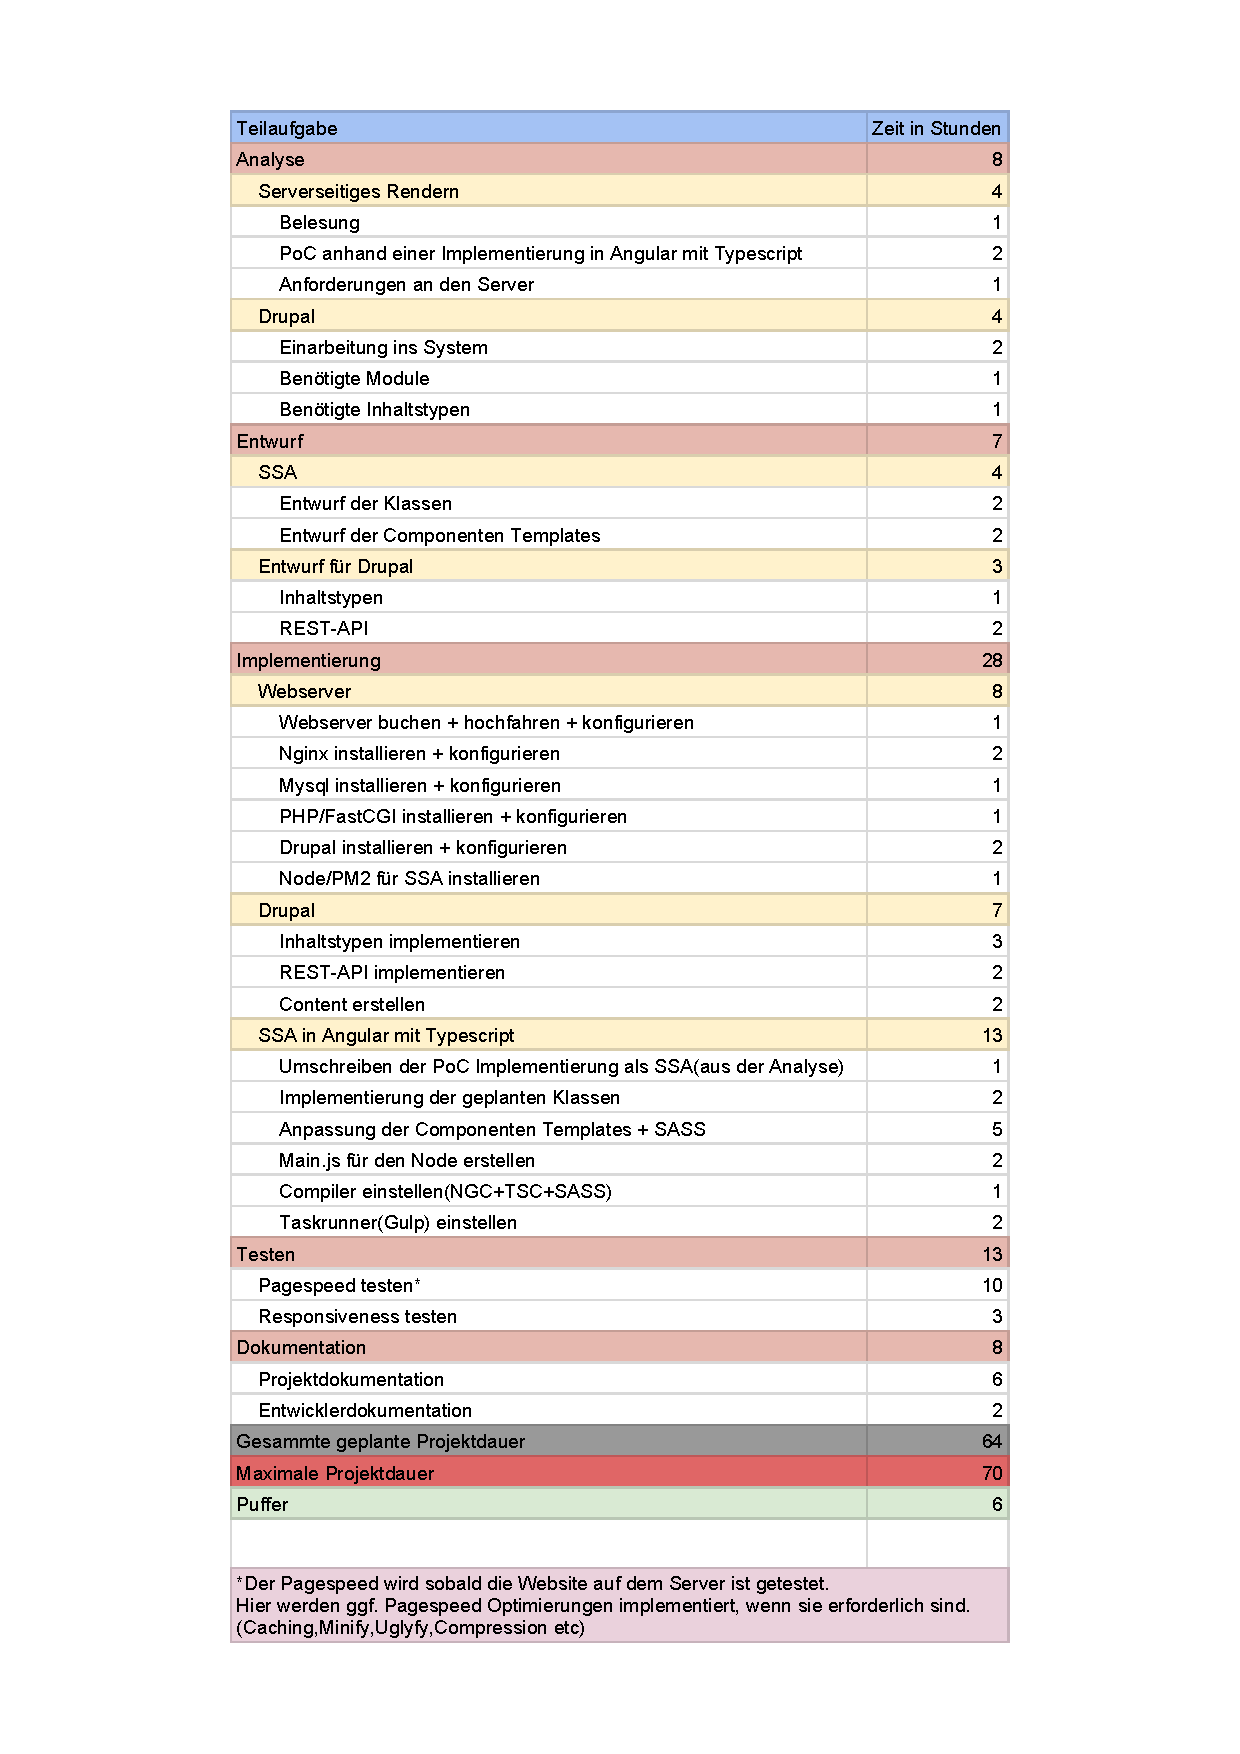
\includepdf[scale=0.8,pages=1,pagecommand=
\subsection{Tabellen}\subsubsection{Detaillierte Übersicht der Aufgaben}\label{sec:teilaufg}]{Teilaufgaben}
\subsection{Grafiken}
\subsubsection{Website Mockup}
\center
\includegraphics[draft,scale=0.1,height=22cm]{Vorlage}
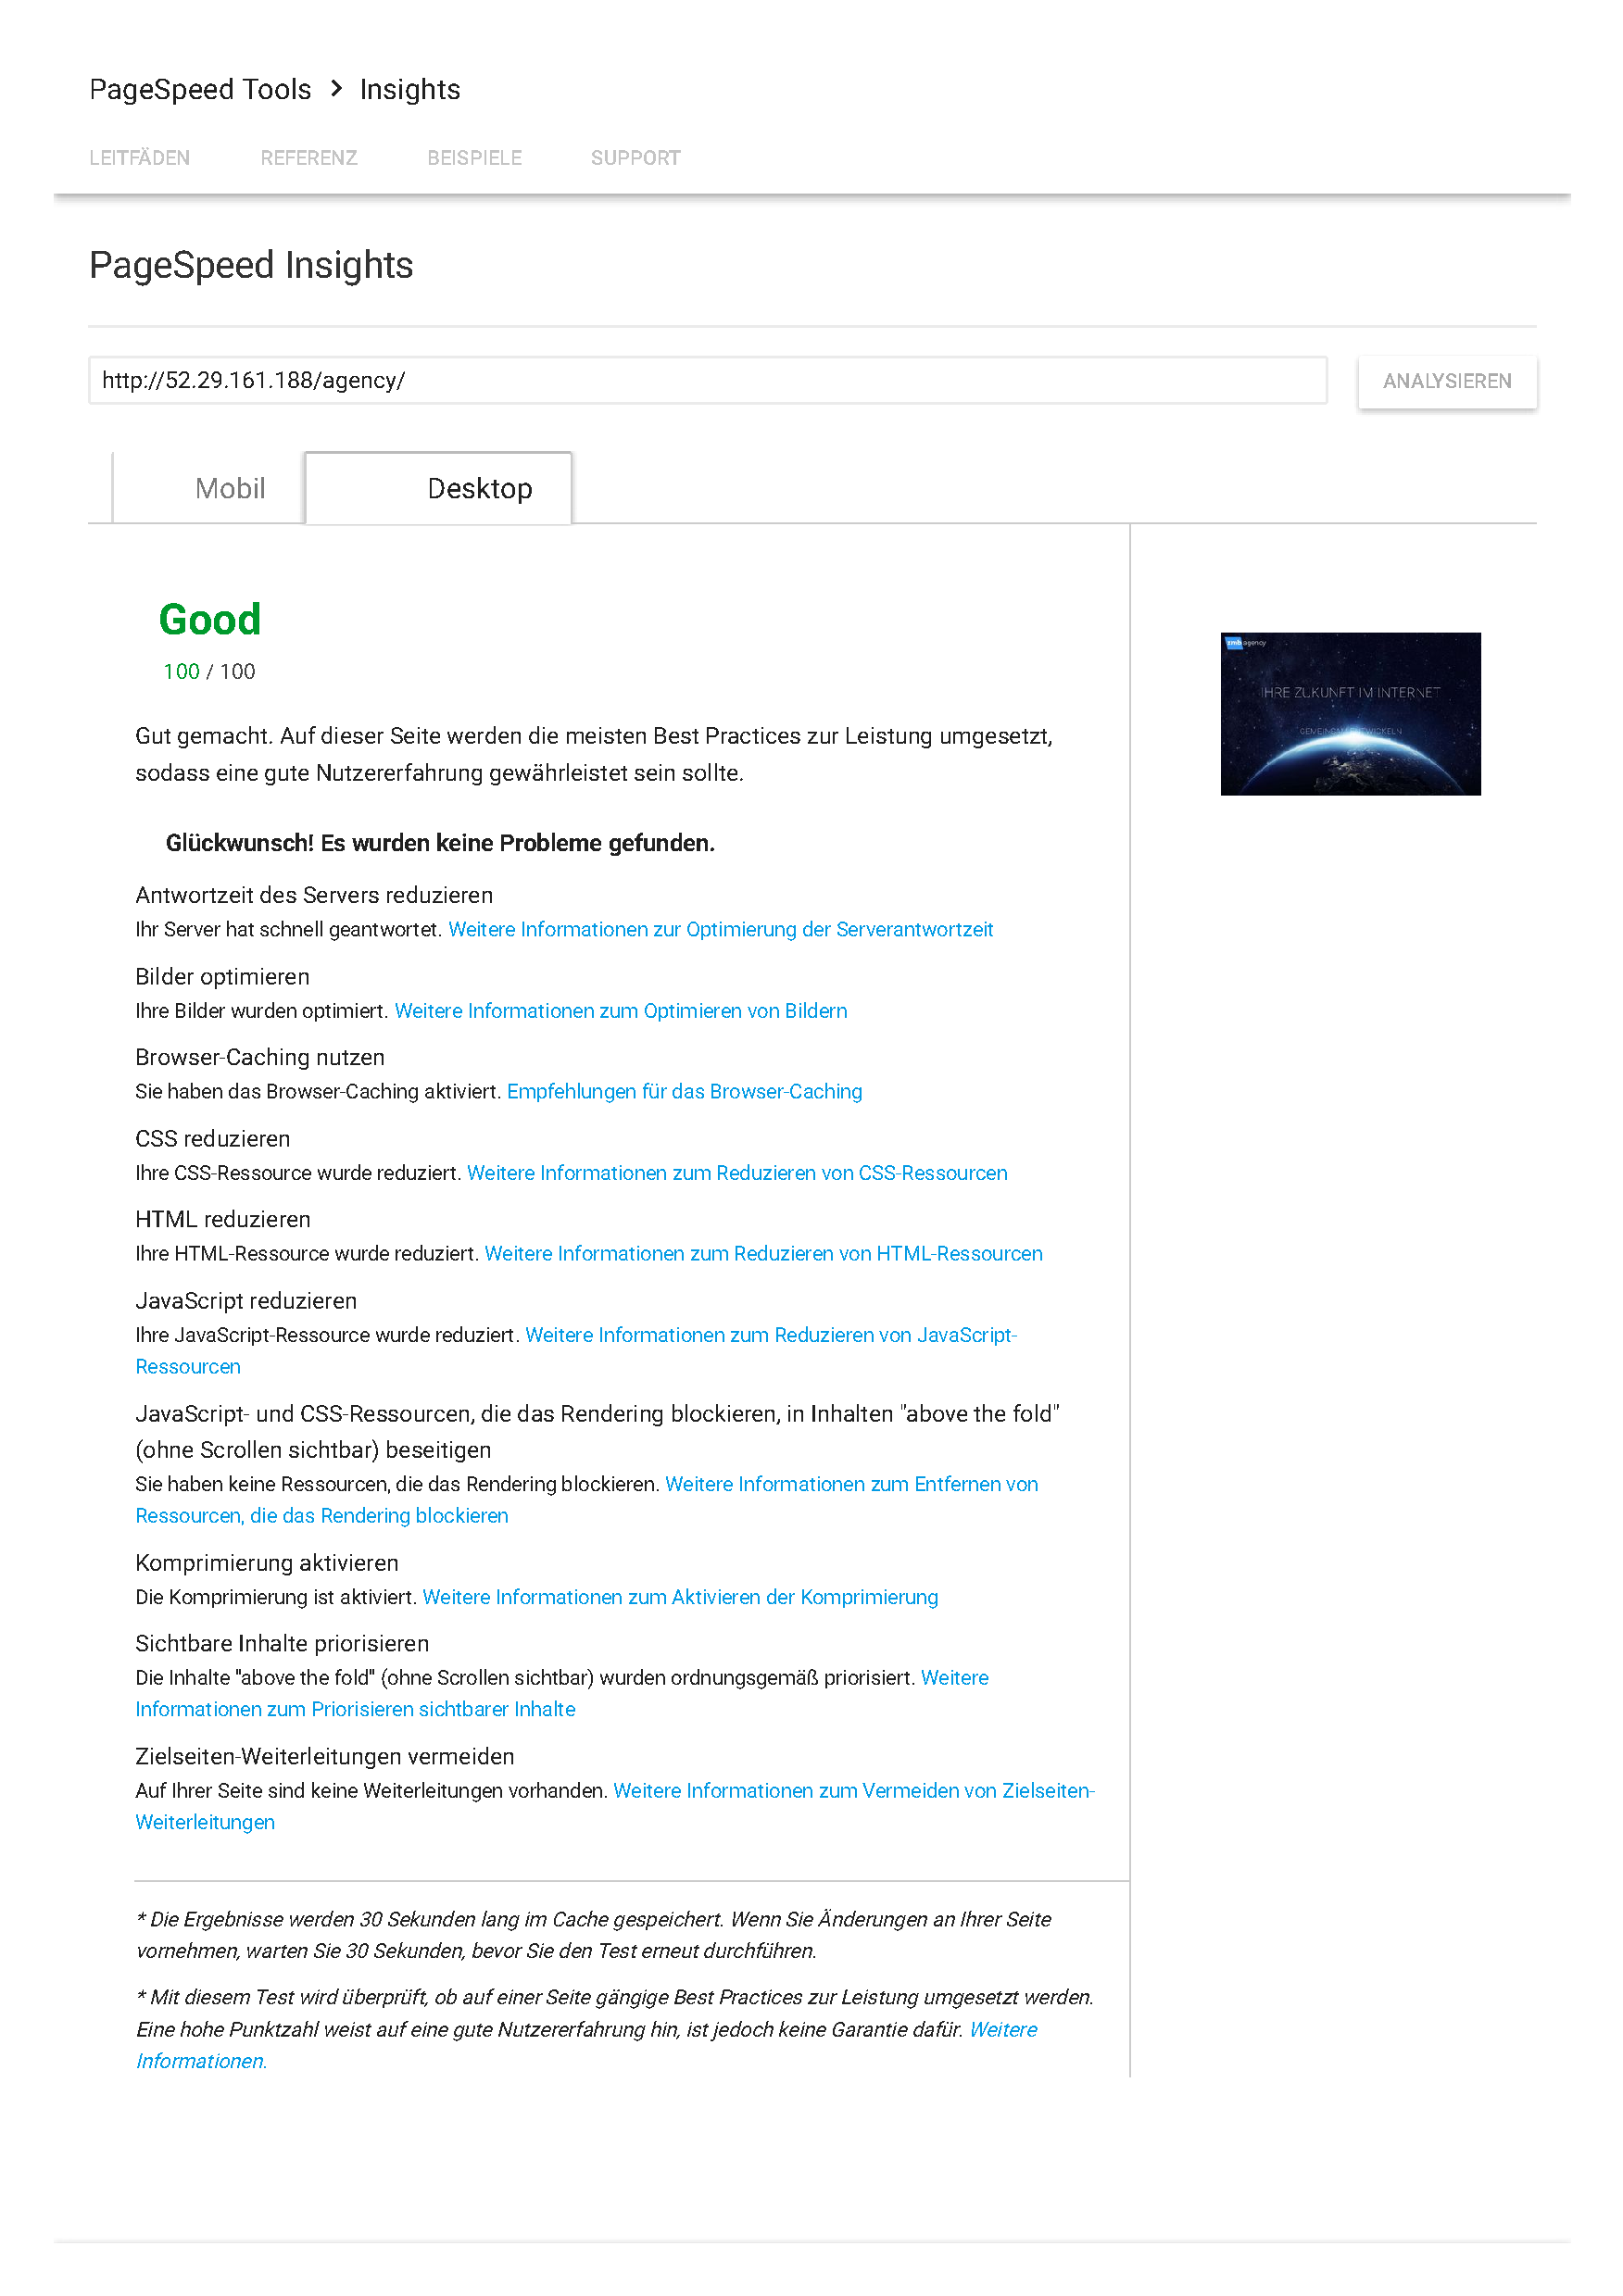
\includepdf[scale=0.8,pages=1,pagecommand=\subsubsection{Google PageSpeed Insights}\label{sec:google}]{pagespeed}
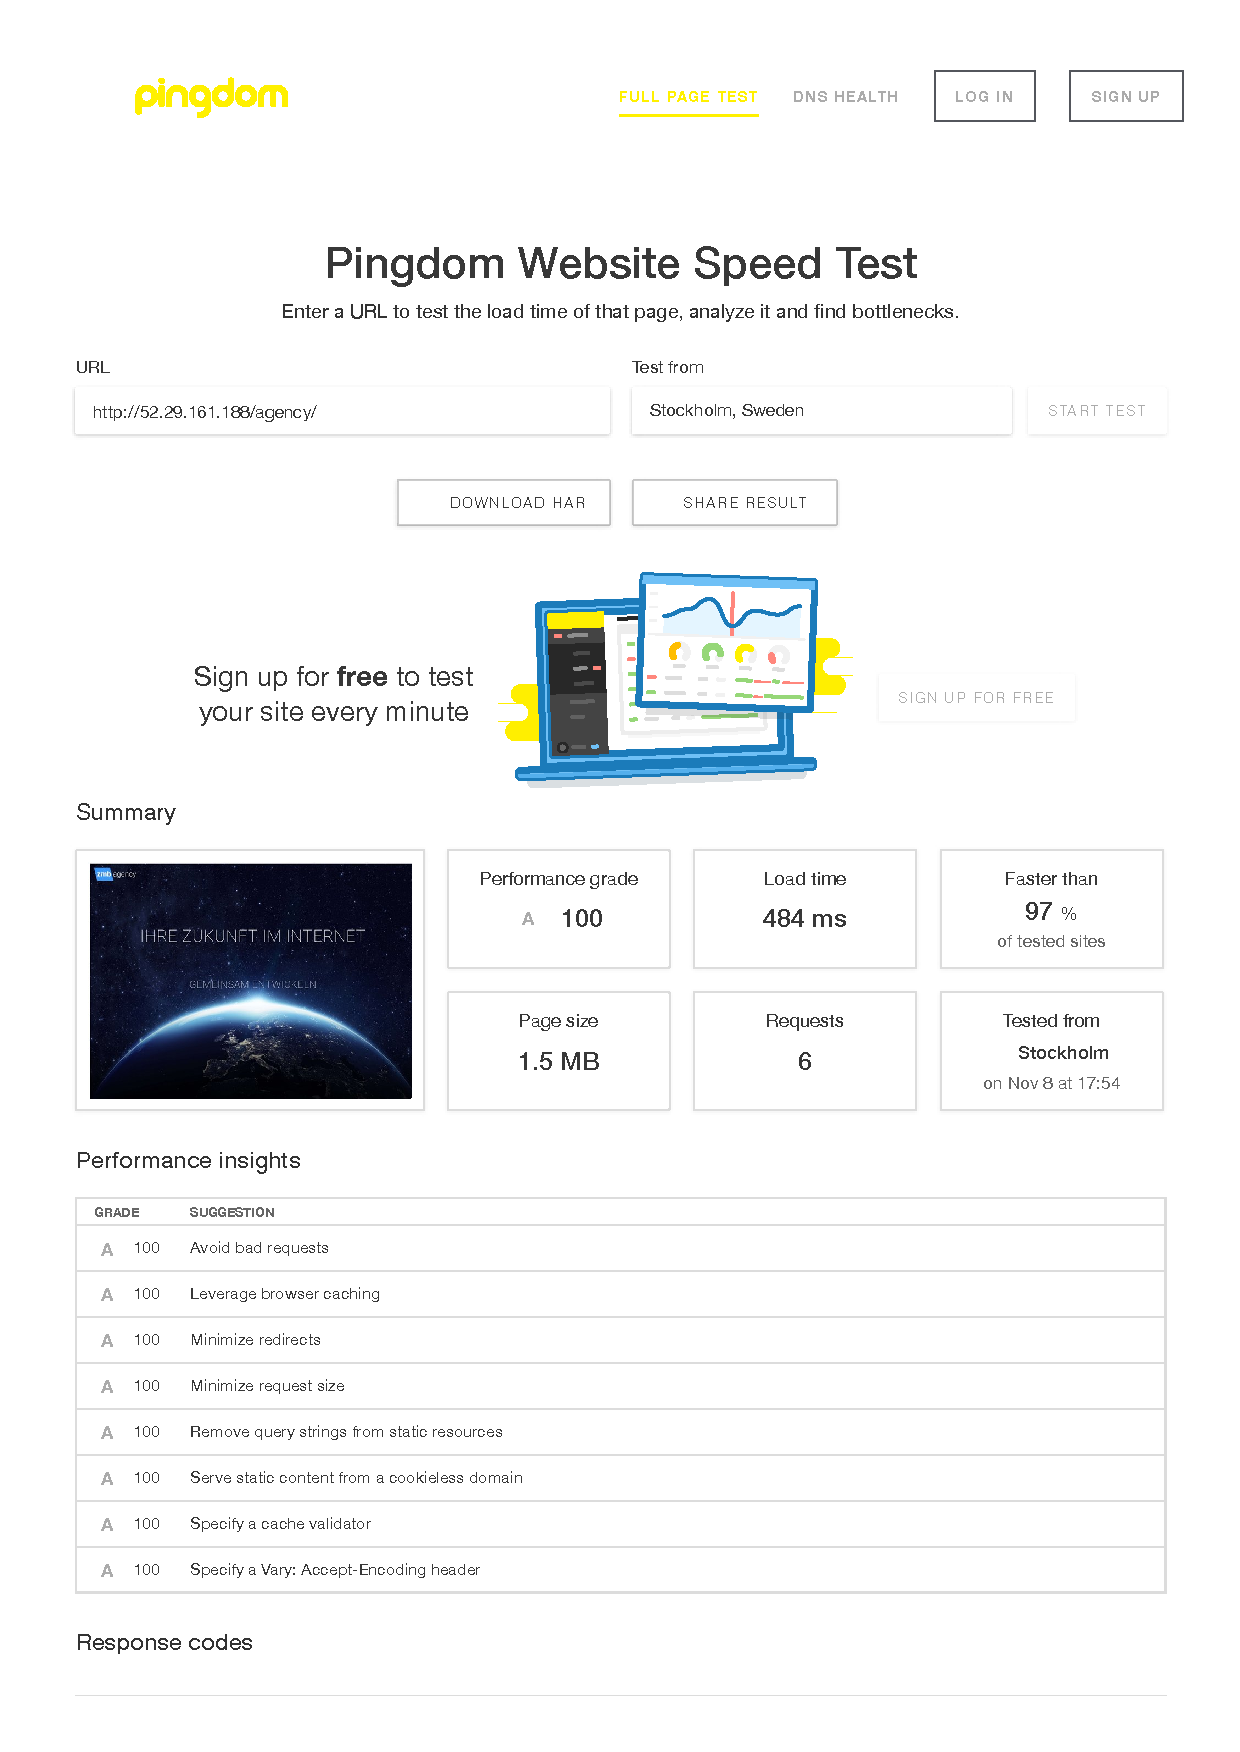
\includepdf[scale=0.8,pages=1-2,pagecommand=\subsubsection{Pingdom}\label{sec:pingdom}]{pingdom}
\subsection{Screenshots}
\subsubsection{Alte Website}
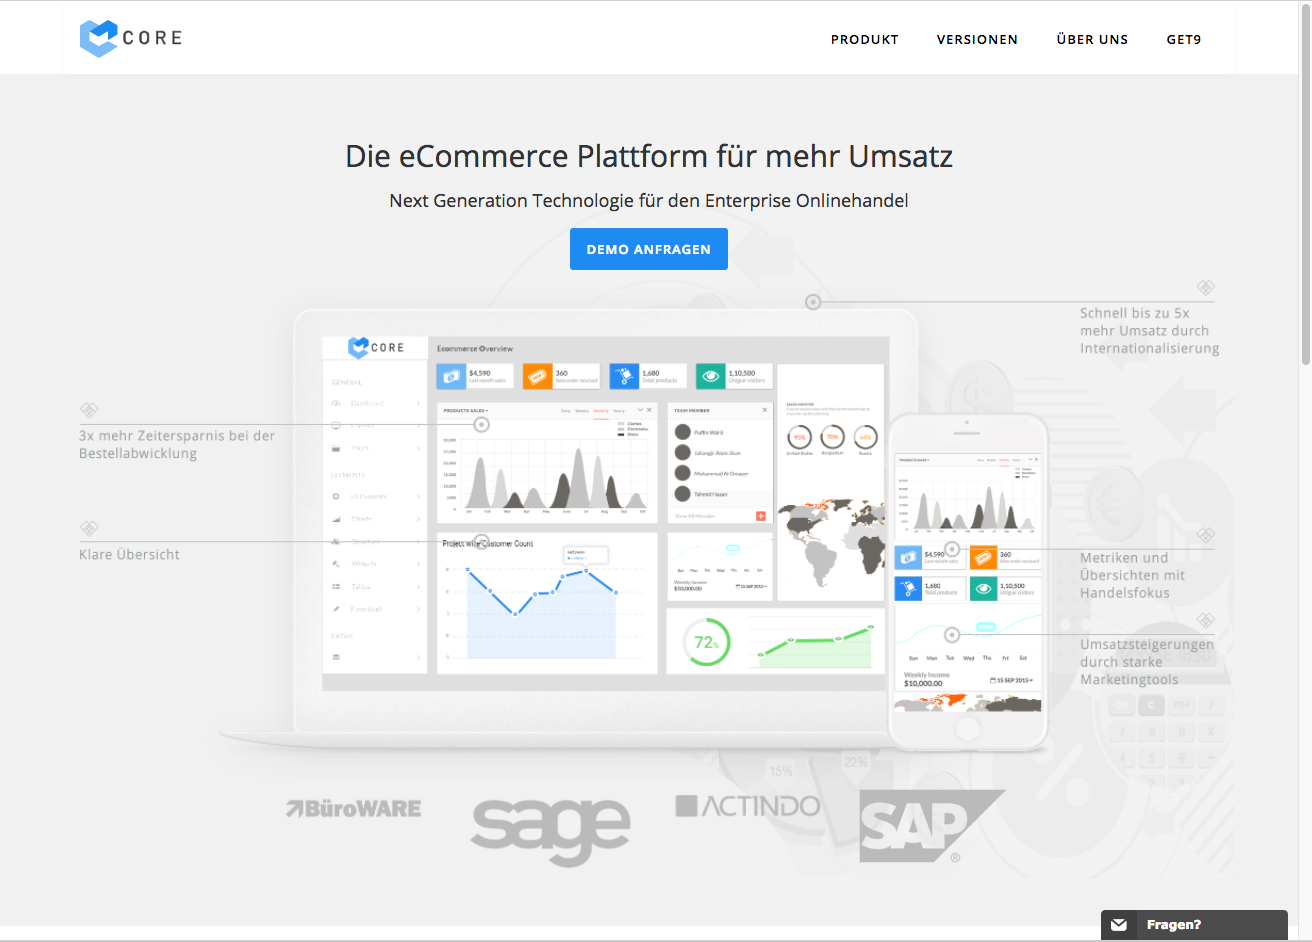
\includegraphics[scale=0.3]{getcore}
\subsubsection{Entwickler Dokumentation}
\label{sec:doku}
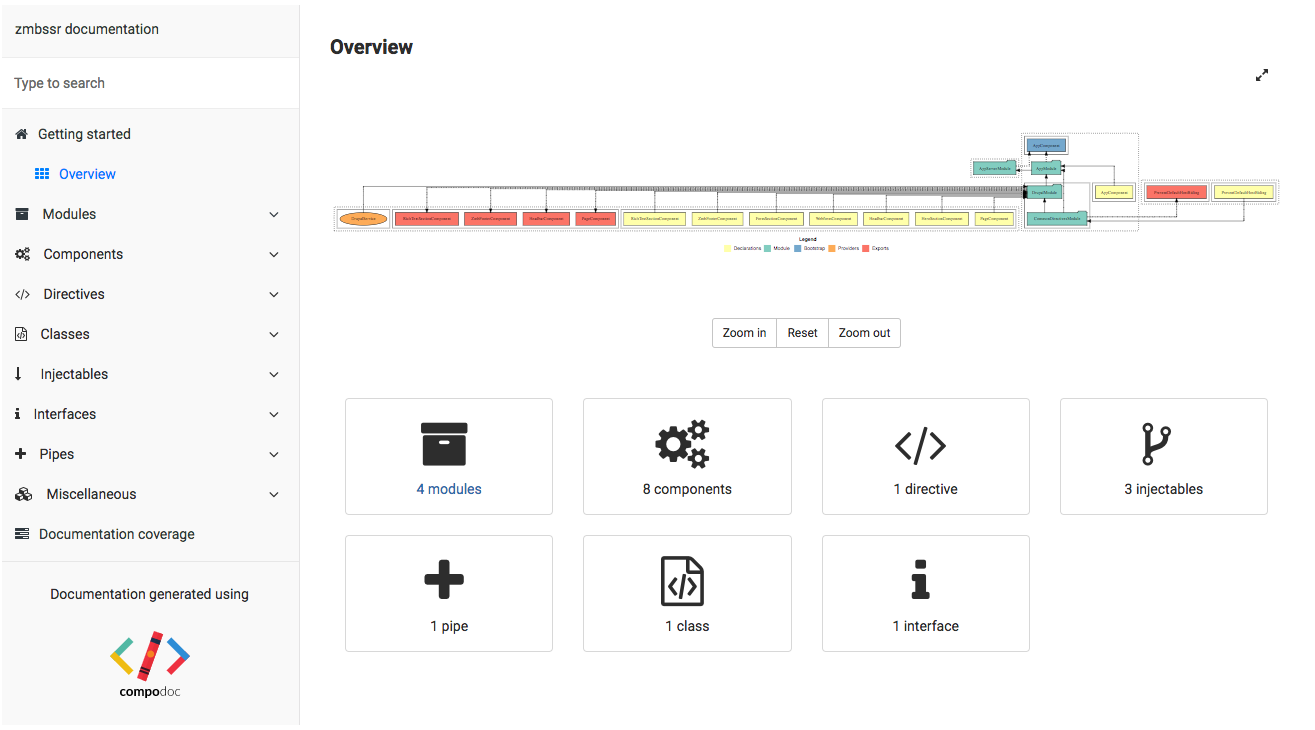
\includegraphics[scale=0.3]{compodoc}

\end{document}
